\chapter{Research}

\label{research}

\section{Introduction}

The use of image processing and its associated computational techniques for the analysis, enhancement, compression and reconstruction of images has been used in the medical domain since the late 1960's and early 1970's to develop an understanding of the processes and composition of the human body \cite{Various2000}. 
More recently, technological innovations in the area of determining body composition accurately have become more mature \cite{Weyers2000} and thus more relevant to the study of the human body as health conditions and the research of disease behaviour has been identified as being dependent on the body's internal composition \cite{Steinkamp1968}. 
Techniques that use MRI scanning or other radiation based techniques offer significant insight into the composition of the body's internal structure. 
Particular studies have utilised whole body MRI scanning to produce images that can then be used to determine composition due to its large coverage, low impact and ability to repeatedly acquire images \cite{Kullberg2010}. \\

Image processing has also been used as a means of calibrating the scanning procedure for patients who require repeated ultrasound or other similar non-intrusive scans of a particular area of the body during a course of treatment or for the diagnosis or analysis of a course of therapy or weight loss programme. 
Previous research has provided the basis for markerless recognition by using points of reference on the human body for automated feature extraction \cite{Iat-FaiLeong2007}. 
The identification of components of the human body without markers forms the basis for the research into identification of sites for ultrasound scanning without the use of significant cues or markers.\\

Range Imaging, especially HDR is a relatively new technique being used in the context of image processing. 
Range Imaging produces 2D images with depth cues and while their relative applications in Medical Imaging have been small to date their potential is evident in previous applications outside of the context of medicine with pixel values corresponding to distance from the device already being used in the calibration of patient positioning for MRI scans using range imaging sensor devices.\\

This research section will consider the use of Body Composition in the analysis and diagnosis of medical state and conditions that a patient may be subject to. 
It will consider the current standards for the determination and analysis of Body Composition and what the future direction of image processing for the determination of body composition is.
Markerless recognition in the context of scan registration and patient calibration will also be explored and technologies and practices identified where the standards are implemented. 
Range Imaging techniques and devices will also be introduced within the context of these previous two medical sub-domains in order to inform our research into related work and project design and implementation.\\

\section{Body Composition}

The composition of the human body as determined by the physical fitness of a person is the relative percentages of fat, muscle, bone and other tissues in the body. 
This ratio of muscle to fat tissue is typically responsible for the outward appearance of a person and determines their leanness with respect to their body fat percentage. 
Body mass and volume is most commonly determined using the Body Mass Index (BMI) and this measurement has been used in clinical trials for a number of years in the determination of health conditions and disease proliferation linked to a person's height and weight \cite{Flegal2012}. However, BMI is limited by the lack of information that can be gained from the correlation of height and weight in the determination of mass and is unable to detect excess body adiposity of people in the intermediate range of the BMI scale who may have reasonable weight to height ratios but excessive weight distribution or abdominal volume. \\

There are 2 commonly used models for assessing body composition. The \emph{2 component model} by Siri and Brozek \cite{SiriAndBrozek} divides the body into a fat component and a fat free component with assumptions made about the constancy of the density of the body and the hydration fraction of the fat free mass. The fat free component exists of bone, muscle and organs in the body. As a means for determining body fat percentage and volume, the 2 component model provides a straightforward means of determining body fat using the \emph{Siri} equation. Importantly, the validity of the 2 component model has been called into account in cases where patients are of an enhanced age or different ethnicity \cite{Guerra2010, Wagner2001}. The 4 component model follows on from concept of dividing the body up into its respective parts but is less commonly used due to the additional complexity of the processes involved in accurately measuring not only fat content but also water, protein and mineral content. Further discussion of the 4C model is outside of the scope of this report. 

\begin{figure}[t]
\label{bmi30}
	\centering
	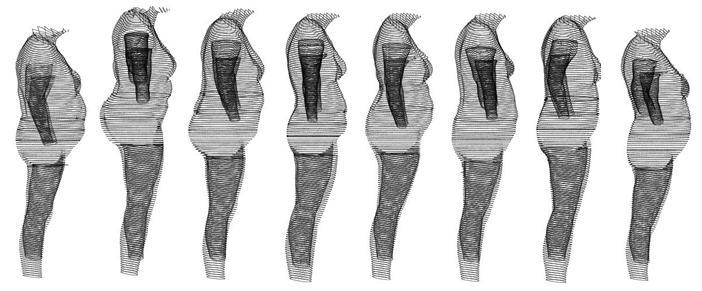
\includegraphics[scale=0.6]{images/bmi30women.JPG}
	\caption{8 Women with a BMI of 30 but with different weight distribution}
\end{figure}

\subsection{3D Photonic Scanning}

A new measure of body composition is the Body Volume Index (BVI) launched in 2010 as an improved anthropometric measurement for the discovery of weight information and distribution on the human body. BVI is ascertained using a 3D scanner to calculate measurements and risk factors that could be associated with a person's body shape and type through the capturing of their weight, volume and body fat. These 3D scanners typically use an array of cameras in a configuration which allows for the capture and rendering of the body so that volume can be calculated. These scans are typically captured under ideal control conditions imposed on the patient such as lighting, pose and restriction on the degree of patient movement. \\ 

The calculation of a person's Body Volume Index in cases of obese patients with moderately high volume readings correlated against the increase of bio markers of cardiovascular disease. This  highlights the benefits associated with methods of acquiring 3D images of the body in the motivation of measuring patient volume for weight monitoring and control purposes. The use of 3D scanning of patients is also suitable where the gross body composition of a patient may deem other means of volume measurement unsuitable. However, the calculation of Body Volume in the diagnosis and prognosis of abnormal body composition in patients has so far remained experimental and hasn't resulted in widespread acceptance by the medical community. This is partially due to the expensive nature of the body scanning equipment, where high specification scanners require 32 cameras, 16 sensors and trained operators \cite{BVIAcceptance}. \\

\subsection{Densitometry}

The Archimedes principle that the volume of an object is equal to the object's loss of weight in water with appropriate correction for the density of the water, has been used as a means for determining the volume of patients since research began into its use as a means to determine patient density in the late 1960s \cite{katch1967} .To this day, the use of this principle is still considered the `gold standard' \cite{anderson2012} when estimating body volume with an average error of 1-2\% under ideal conditions over repeated intervals \cite{Rolland2012}. \\

\subsection{Air Displacement Plethysmography}

Hydrostatic displacement, or air displacement, uses the same principles of densitometry but measures the displaced air within a known volume of air using the ideas of plethysmorgraphy. A plethysmograph measures changes to volume within an organ or in an entire body. In studies, air displacement plethysmography has been used for the assessment of body composition in children and adults. The BOD POD, a hydrostatic weighing chamber, is considered the only commercially viable implementation that is used for this purpose \cite{Fields2004}. \\

\begin{figure}[t]
\label{2c4cerror}
    \centering
    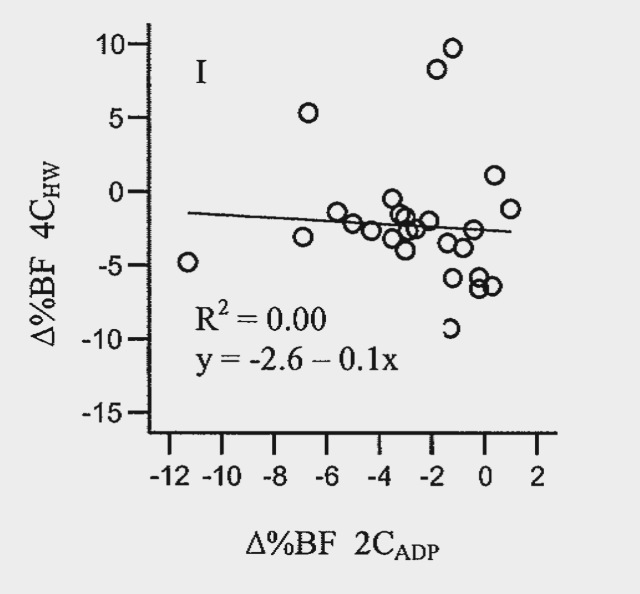
\includegraphics[scale=0.4]{images/2c4cgraph.png}
	\caption[Changes in \% body fat, comparing Bod Pod to a 4-compartment model]{Changes in \% body fat, comparing Bod Pod to a 4-compartment model. R=0 represents no correlation between these composition measures over time.}
\end{figure}

Patients enter into the chamber which consists of 2 sub chambers with approximately 300-400L of capacity. A diaphragm moves between these chambers creating sinusoidal volume perturbations which result in very small pressure changes that can then be detected by transducers in the hull of the primary chamber in which the patient sits. This measurement takes place in non isothermal conditions and the volume measurement recorded taking into account the surrounding pressure in the chamber using Poisson's law. Poisson's Law states that $\gamma$ is the ratio of the specific heat of the gas at constant pressure to that of constant volume and is equal to 1.4 for air and p represents the pressure in each chamber. \\

\begin{equation}
    \label{eq:poissonlaw}
    P_1/P_2 = (V_2/V_1)^\gamma
\end{equation} 

These pressure changes are subject to error if the chamber itself is improperly sealed, if the patient moves or breathes irregularly or has significant pulmonary activity. It is also poor for measuring changes over time as each scan is subject to a number of variable factors such as humidity and what the patient is wearing.\\

However, statistically significant variations of the volume measurement of a single patient over time, even where elements of the scan are tightly controlled, such as breathing; environment and clothing, have been observed. This has meant that the relative error between the 2 models of measurement mean that measurements over time have shown little to no correlation of the volumes captured \cite{Mahon2007}. This has caused some academics to call for further research into the issues surrounding the two compartment body composition approach where a 4 compartment model may be more accurate. The inaccuracies of the air displacement  methodology that the BodPod advocates may be due to the assumptions made by these models \cite{Lifemeasurement1997}. \\

\subsection{Limb Circumference}

Aside from these technologies used for the reconstruction and evaluation of body volume, the role of limb circumferences as a reflection of body composition should not be overlooked. The distribution of muscle density and subcutaneous fat deposits manifests itself around particular areas of the body. Measuring the circumference can give a reasonable idea of the changes to muscle and fat composition in limbs over time \cite{Frisancho1981}. These areas are often measured and monitored in order to aid in the prognosis of particular conditions or treatment plans. \\

Conventional measurement makes use of spring tape or skinfold calipers. Martin et al highlight the need to take several measurements when using calipers due to the variability of adipose tissue patterning in areas of the body. Strict guidelines govern caliper usage making it susceptible to error \cite{Martin1985}. The application of image processing to this domain is apparant in localized MRI scanning where the composition of these areas can be analysed for body fat ratio and estimation of circumferences across the body; MRI however is costly and often inaccessible for such means \cite{Reeves2004}. \\

\begin{figure}[t]
\centering
        \begin{subfigure}(a)
            \label{volLED}
            \centering
            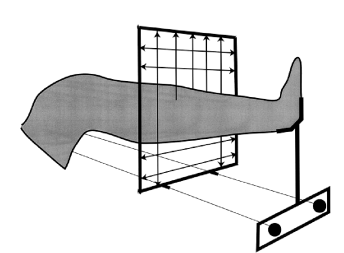
\includegraphics[scale=0.4]{images/volumetry.PNG}
            \end{subfigure}
            \begin{subfigure}(b)
                \label{volWATER}
                \centering
                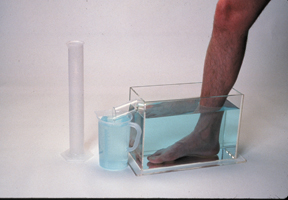
\includegraphics[scale=0.4]{images/waterdisplacement.jpg}
        \end{subfigure}
        \caption{Volumeter configuration for scanning the lower leg (left). Conventional water displacement method on (right).}
\end{figure} \\

Technology that does not use direct limb circumference measurement but rather extrapolates it from a given volume has been shown to produce accurate anthropometric measurements for each limb. The volumeter captures the volume of local limbs using an array of infra-red sensors. These sensors capture the contours and overall volume of a limb and this gives its equivalent circumference. Heinz et al found a $0.60$ average variance from the spring tape measurement and under ideal patient setup, provided an effective means of monitoring changes in volume and circumference of limbs \cite{Heinz2000}. A clear drawback in the majority of these technologies is the required setup and calibration required for such equipment \cite{Bauer2011}.\\

There is little research to suggest that a range imaging implementation with little previous calibration or setup would be suitable nor unsuitable. The work of Heinz suggests that circumference calculations that use volume-based estimation are likely to be biased towards larger estimations when compared to spring tape, although the error is evaluated as not significant to the overall accuracy of the method, and the relationship between them, postively linear \cite{Heinz2000}. \\

\section{Range Imaging}
\label{res:range imaging}

Intensity images such as MRI scans or heat maps applied to a scene based on a specific criteria related to the environment (such as temperature or humidity) do not impart much information about the surfaces they capture so estimating or inferring details from such images is limited. Range imaging encodes the positions of surface geometry directly so that the captured scene can be captured in terms of a depth map that can then be visualised. These images can be expressed in terms of a list of 3D coordinates in a frame or a sequence of frames with no strict ordering in the coordinate space. They can also be represented in terms of a matrix of depth values along the directions of the x,y image axes imposing a strict ordering on the points as a result \cite{Helmut2002}. Proper calibration of the equipment can yield distances in terms of standard metrics useful for calculating distances or heights in real time similar to the operation of LIDAR \cite{Maltamo2006}. 

%what each thing is and it's advantages/disadvantages

\subsection{Technologies}

Devices that produce range images can consist of a single camera, an array of cameras or a camera that is used in conjunction with a sensor array that is capable of capturing the depth information of a scene. Some of these technologies exploit the nature of the focal point or aperture in the device itself while others rely on the use of light both in the UV spectrum and outside of the visible plane.

\subsubsection{Stereo triangulation}

Stereo triangulation uses the concept of triangulation, determining a point in 3D space given it's projection onto $n$ images. Triangulation is achieved by identifying the camera projection function by which the 3D scene is projected onto 2D space. In the simplest case, this achieved using the camera's specific transformation matrix for achieveing this projection. By making this triangulation stereo, we are able to reconstruct a scene over the subset of points that the camera can capture. A simple triangulation method, $x \sim \tau(Y_1,Y_2,C_1,C_2)$, where $y_1$ and $y_2$ represent the homogeneous co-ordinates of the detected image points, $c_1$ and $c_2$ represent the camera transformation matrices gives $x$, the homogeneous representation of the 3D point. This method doesn't require specific illumniation conditions but requires that there is maximal correspondence for a given point captured by the cameras. This is made difficult due to the noise and geometric calibration inaccuracies that may result from a typical configuration \cite{Hausler1993}. \\

This method is also viable where a `plentopic camera' or single lens camera is used and reduces the overheads surrounding correspondence between image sensors in a binocular camera configuration. The use of this configuration was successfully used by Adelson in their replication of single lens stereo through the use of a plentopic camera \cite{Adelson1992}. They captured the structure of the optical light that hit the camera lens thus analysing the amount of light at each part of the scene allowing them to capture depth information from the virtual displacements achieved from their analysis of light hitting the optic lens. This particular method is only really suitable for achieving a depth map at a close range to the object rather than an entire scene due to the size of the lens aperture. Stereo triangulation remains widely used in the domain of robotic computer vision especially in the context of explorative robots that use SLAM (Simultaneous Localization and Mapping).

\subsubsection{Time-of-flight (TOF)}

Time of flight range imaging uses TOF cameras to capture a scene based on the notion of the known quantity of the speed of light. This is primarily done by measuring the speed at which light hits a particular point of a scene and then bounces back to the imaging sensor as a form of scannerless LIDAR, in this sense it is very similar to the operation of the Structured Light approach or the Microsoft Kinect but has the added algorithmic complexity which means that Time of flight camera's can also capture depth changes as they occur in real time, or relatively high resolution video frame rates (24fps) and it can be integrated into a configuration which allows for fast object capturing \cite{Cui2010}. Local rigid alignment between scans  is also possible using an Iterative Closest Point (ICP) algorithm. The passive nature in which Time-of-flight cameras capture scans is subject to a degree of noise and `Systematic bias'. This bias can lead to non-rigid scan distortions which affects the overall registration of the images captured by the camera. The distortions result from the 3D point measured by the depth camera being different from the orientation of the camera ray toward the point. TOF cameras are also expensive and require additional sensor arrays to operate accurately and effectively. 

\subsubsection{Coded Aperture}

Coded Aperture aims to retrieve raw depth information from a conventional RGB image captured using normal camera apparatus. This is achieved through measuring the colour intensity of the RGB image. The purpose of coded aperture is not to recreate a scene digitally nor achieve refined depth information for each point in the scene but to provide a cue for extended depth of field or markers for depth-based image editing. Levin et al in use a coded apeture to filter the image sensor so that the incident light on the camera lens is coded such that depth information can be extracted from the resultant image. The capturing of this depth map is useful where the focus or blur for a particular image is based on the referent of the depth map. It means that at the post processing stage, we can affect the image's focus using the depth map so different focus points can be yielded based on the information captured by the depth map. While this technique only works on still images and lacks the finer detail required by the 3D reconstruction of objects or an environment. 

\subsubsection{Structured Light}

This method uses a specific pattern of light which is ideally projected onto an object which is then captured by a camera or array of cameras. The most common pattern used is a series of strips projected onto a surface, the deformation and displacement of the projected light beams on the surface means that a typical configuration will be able to identify geometrics positions in 3D anywhere on the object after a sufficient number of captures have been taken as the structured light pattern converges to finer intervals. This structured light approach gives high accuracy stereo depth maps and in the majority of cases gives pixel-accurate correspondence between the subject captured the point registered in 3D space \cite{Scharstein2003}. The benefit of using stereo based depth maps is that the correspondences between the two images can be registered immediately without the requirement for further post processing. \\

Because of its accuracy and quality of the depth maps it produces, structured light mechanisms are frequently used in 3D Body Scanning configurations. Such a context yields accurate models of depth as their is only a single object of focus with which highly accurate displacement of light can be recorded. However, when applied to scenes with additional complexity containing a number of objects at different depths, Scharstein et al \cite{Scharstein2003} found that several small areas in a more complex scene shadowed under various types of strip illumination giving unknown disparities in the final depth map. Structured light is also poor for giving real time depth representation in fast moving scenes due to the low refresh rate inherent in the design of the algorithm.

\begin{figure}[ht]
\centering
        \begin{subfigure}(a)
            \label{lightscanner}
            \centering
            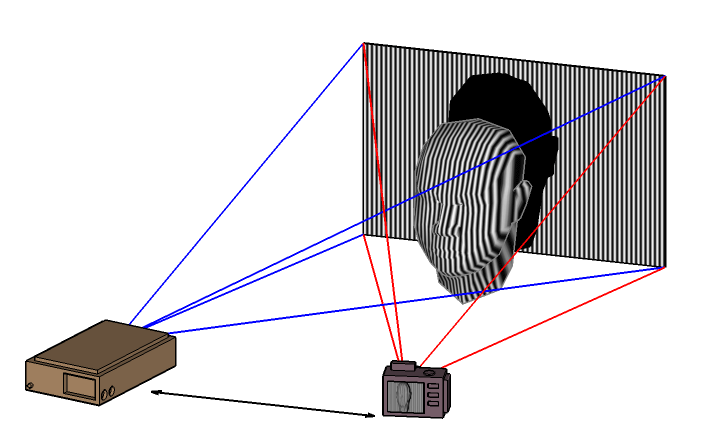
\includegraphics[scale=0.3]{images/structuredlightscanner.PNG}
            \end{subfigure}
            \begin{subfigure}(b)
                \label{shadowing}
                \centering
                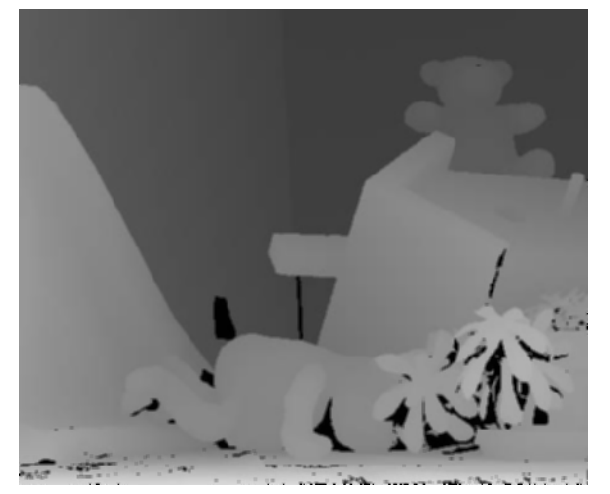
\includegraphics[scale=0.3]{images/occludedareas.PNG}
        \end{subfigure}
	    \caption{Typical structured light scanning configuration. Image on right shows shadowing in the depth map.}
\end{figure}

\subsubsection{The Kinect}

%include images, talk about the advantages/disadvantages of the device.

The hardware that The Kinect, originally a gaming device designed for the Xbox 360 gaming console, features is based on the principles of structured light as well as using aspects of stereo triangulation for the calculation and relative mapping of distances in a depth map. The Kinect projects a fixed pattern of infra-red dots onto a scene using an IR projector. Using a monochrome CMOS, the distance of each IR dot on the scene from the Kinect is captured and then post processed into a depth map. The benefit of having a fixed IR pattern means that the changes in the displacement of each of the fixed points can be recorded as subjects move in the scene. This allows for higher capture frame rate as the position in the x,y plane is maintained with only measurements in the z plane needing to be updated. This also means that calibration only needs to happen at the start of the capturing process or if the device is moved. \\ 

The Kinect also benefits from the use of the Kinect for Windows SDK \cite{SDK13}. The latest revision of the SDK (1.7 as of March 2013) includes support for the capturing and development of interactions such as those you would expect from a touch screen device. It also includes support for coarse spatio-temporal reconstruction of the scenes and objects that the camera captures using KinectFusion. The hardware as well as the inclusion of a stable established API provides accessible range imaging technology for developers and researchers, where traditional range imaging technology is out of reach due to the difficulty in achieving ideal scanning configurations or the overall initial cost. \\

\begin{figure}[ht]
\centering
        \begin{subfigure}
            \label{fig:kinectoffset}
            \centering
            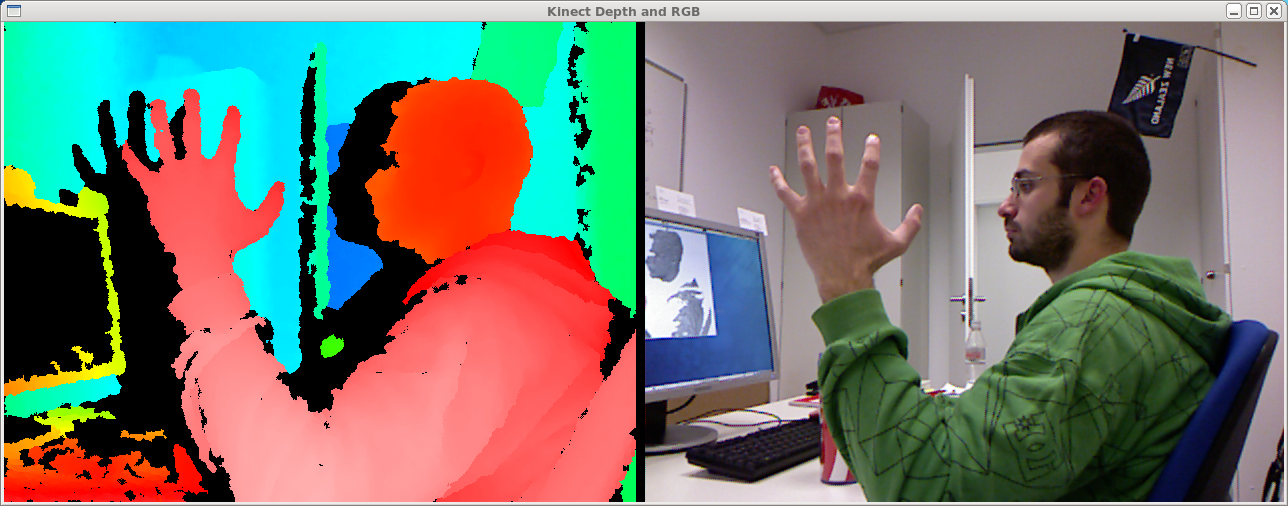
\includegraphics[scale=0.15]{images/kinectoffset.png}
            (a)
            \end{subfigure}
            \begin{subfigure}
                \label{kinectrecon}
                \centering
                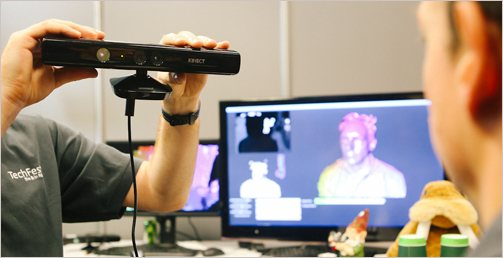
\includegraphics[scale=0.515]{images/kinectfusionrecon.jpg}
            (b)
        \end{subfigure}
        \caption{\emph{Top: }showing RGB and Depth Map with 10-20mm offset. \emph{Bottom: } non-rigid capture of human subject using Kinect SDK.}
\end{figure}

As observed in \ref{fig:kinectoffset}, the accuracy of the Kinect depth data is subject to the offset that exists between the RGB lens and IR receiver on the device. This offset manifests itself as an acute shadowing that forms due to the inaccurate orientation of the RGB camera with respect to the depth co-ordinate system. Further experimental results by Khoshelham's investigation \cite{Khoshelham2011} into the accuracy of depth data generated by the Kinect shows greater error registered the larger the distance due to the low resolution of depth data recorded at these distances \cite{Khoshelham2011}. The point clouds generated by the Kinect and that of a higher resolution laser based scanner recorded up to a  4cm discrepancy at larger distances. These point clouds were then subject to a registration exercise. The systematic error discovered in the point cloud pair generated by the Kinect demonstrated a greater error in plane registration compared to the laser based scanner. While the point density recorded by the Kinect was found to be lower than that of a laser scanner; a point cloud captured under ideal illumination conditions with sufficient calibration demonstrated only a small systematic error when compared to the laser based point cloud.



\section{Skeletal Pose Estimation}

Skeletal Tracking, even though not directly related by itself to the aims of the project, is part of the base functionality needed for the development of all core components. Skeletal tracking and pose estimation is achieved by the Kinect Skeletal API, which uses the Kinect's depth feed.\\

Detecting humans, possibly in different poses, has been an interesting point of research in different areas. Aiming to detect human activity in real time, A. Argyros and M. Lourakis \cite{Argyros2004}, developed a method for tracking multiple skin-coloured objects, which could represent human parts such as the face and the hands. Simply using colour detection raised some issues when detecting different body parts intersecting with each other, as they could be interpreted as a single object. This issue was addressed by detecting each object as it entered the field of view of the camera and assigning a unique label to it, while maintaining the labels of previously detected objects. The method was able to track multiple moving objects moving successfully and it was also able to cope with complex movements and detecting the entry and exit of objects from the field of view of the camera almost instantly. Even though this method could detect body parts in detail (such as detecting the fingers as part of the hands when the palm was open) it did not however include any recognition of what the body parts were or any inference of the rest of the body.\\

Following a different path, looking into 3D human pose reconstruction, Kanaujia et al. \cite{Kanaujia2007} use a human pose prediction algorithm. As opposed to previous suggestions, the algorithm performs the prediction directly based on the image, rather than by searching a pose space looking for cases with good image alignment. Distinguishing between slightly different poses or detecting poses that were similar but in different circumstances, such as people with different body-types or different background and lighting, was challenging. To overcome these difficulties, the method implemented used “bags of features”, which helped differentiate between poses based on specific features that the poses included, such as angles of joints.\\

Going one step further, Shotton et al. \cite{Shotton2011} use a single depth image and attempt to estimate the  3D positions of body joints. They however approached the pose estimation problem by using object recognition instead, to distinguish between the different body parts. Following that, a per-pixel classifier is used that is trained enough to be accurate despite pose, body-type or other differences between the images. The result of the classification is used to generate 3D joint proposals. Similarly to the first example, this method labels body parts already recognised but, extending that, it uses the labelled parts to infer other parts that are missing by using an intermediate representation.\\

Shotton et al. continue their research by extending it to predict 3D joints in real-time and managing to achieve it without the resource-consuming intermediate body-parts representation, but straight from the depth image \cite{Girshick2011}. Since they have already covered pose recognition from a single image in their previous research, they use many single frames rather than sequences. They also extend their synthetic training data set to cover a wider range of body shapes and their true joint positions for 16 different joints.\\

These findings by Shotton et al. formed the basis for the skeletal tracking technology that is currently used with the Kinect \cite{Zhang2012}. The operational demands for this research were huge, as creating such a commercial application implies several additional requirements, such as the fact that it should be able to perform equally well regardless the person, dimensions of the environment, lighting, tilt angle of the Kinect or distance from it. This should also be done with low usage of resources so that it does not affect the continuity of the application or game it is used with. An important aspect of the implementation that contributed towards the fulfilment of those goals was the inclusion of body-part recognition before pose estimation rather than detecting the pose directly. To achieve these results the per-pixel classifier mentioned above was used, followed by making a hypothesis of the locations of the joints by using the training data set created with forming synthetic depth images with different body-types. The 3D coordinates of the joints are then mapped to the skeletal joints. This is done by continuously taking temporal continuity and prior knowledge into account. The whole process happens in real time to allow for continuous interaction.\\

\begin{figure}
    \centering
    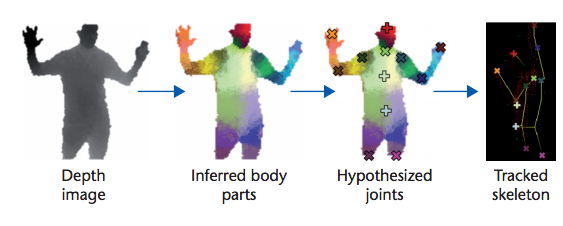
\includegraphics[scale=0.5]{zscreenshots/skeletonJoints.png}
    \caption{The Kinect Skeletal Tracking Pipeline}
\end{figure}

\section{Person Isolation}
\label{testing:person isolation}
This section details the testing of the depth based person isolation.\\

\subsection{Isolating Multiple Subjects}
During the design of depth based person isolation in Section \ref{imp:depth based isolation}, the isolation was determined to be sufficient for one person. Further testing was conducted on multiple subjects to confirm that the method would work on many people, rather than only the subject in Figure \ref{fig:depth and hand based cut off}. Figure \ref{fig:multiple subjects isolated} show the behaviour of the isolation method on the aforementioned multiple subjects. From this figure, the isolation method can be said to work consistently on many subjects.\\

\begin{figure}[h]
\begin{center}
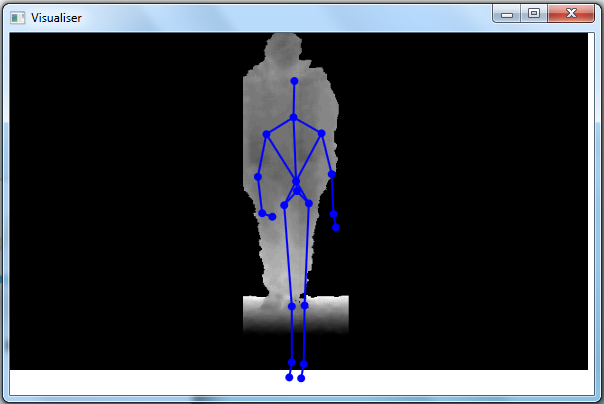
\includegraphics[scale=0.3]{images/bernie_iso} 
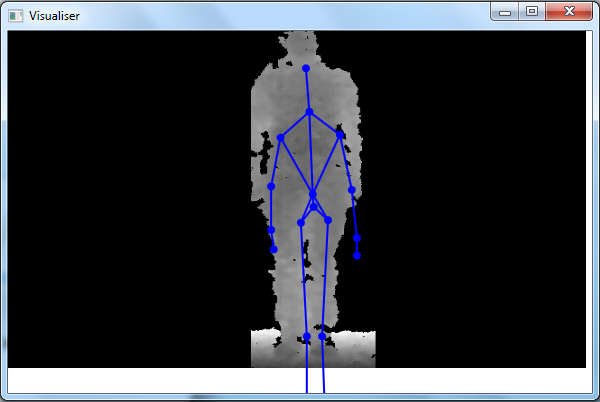
\includegraphics[scale=0.3]{images/page} 
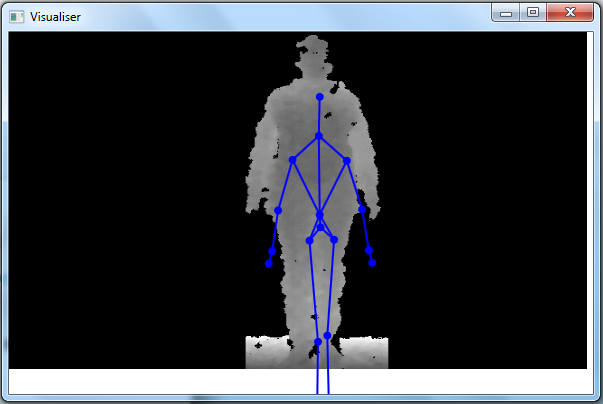
\includegraphics[scale=0.3]{images/steffat} 
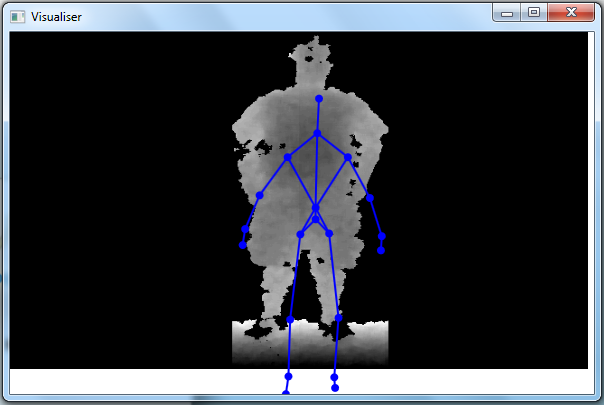
\includegraphics[scale=0.3]{images/wilkoiso} 
\end{center}
\caption{Multiple subjects isolated.}
\label{fig:multiple subjects isolated}
\end{figure} 

\subsection{Floor Removal}
As previous noted in Sections \ref{design:depth based isolation} and \ref{imp:depth based isolation}, the depth based cut off leaves the floor underneath the person as an unwanted artifact in the final point cloud. Fortunately, the floor can be removed at the point cloud level as suspected. An example of this action is shown in Figure \ref{fig:floor removal}.\\

\begin{figure}[h]
\begin{center}
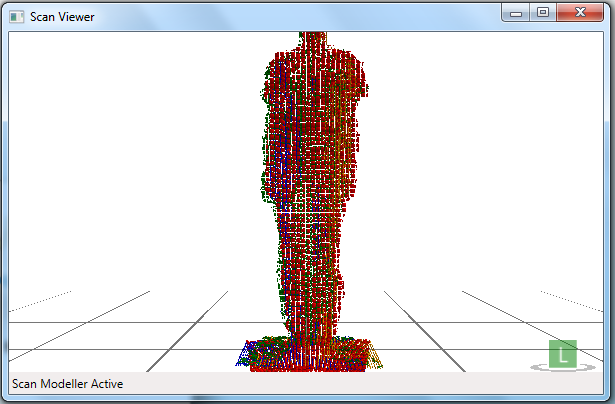
\includegraphics[scale=0.3]{images/greg_feet}
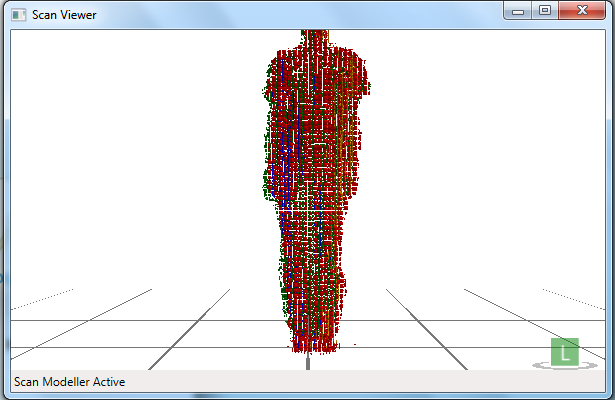
\includegraphics[scale=0.3]{images/greg_nofeet} 
\end{center}
\caption{Left: The point cloud with the floor. Right: After floor removal.}
\label{fig:floor removal}
\end{figure} 

\section{Registration}
\label{testing:registration}
This section deals with the testing of the registration functionality, as described in Section \ref{design:registration}. 

\subsection{Methodology}
Testing this sub-system was not a trivial exercise due to the interdependence with volume estimation. That is, correct volume estimation requires correct registration but the correctness of registration can only be measured by observing correct values of volume estimation.\\

The best way of determining the accuracy of stitching is by analying the deviance of the Toolkit Volume Measurement from the Gold Standard Volume measurement, which can be read in Section \ref{testing:vol est}. The first data point, Bernard, is a control and the error is irrelevant. \\

\section{Volume Estimation}
\label{design:volume estimation}
There are many techniques for estimating an arbitrary metric of a given 3-dimensional shape, including the volume of the shape.
Focus will first be on height estimation to see if the methods can be extended to calculate volume, before moving to methods specifically designed for volume estimation.\\

\subsection{Estimating the Height of Trees}
LIDAR has previously been used to estimate the height of trees from above \cite{Maltamo2006}. Three laser scanning-based methods were used to compute the height of the trees: a direct prediction model for the stem volume at plot level, a volume prediction system based on the modelled percentiles of the basal area diameter distribution and a parameter prediction method used to determinate Weibull based basal area diameter distributions \cite{Frechet1927} for the plot-level stem volume prediction. The best results were obtained with the first method, i.e. the model that predicts plot-level stem volumes directly \cite{Maltamo2006}.\\

In order to calculate the height, the laser reflections from non-ground objects, such as trees and buildings were classified as non-ground hits using TerraScan software \cite{Solid2013}. Conversely, other points were classified as ground hits. Canopy height of a non-ground object is then calculated as the difference between the height of the non-ground object and the neighbouring ground points. The accuracy of this method was found to be better than $\pm$15cm \cite{Maltamo2006}, when compare to field-measured volumes obtained with the Finnish conventional method Inventory by Compartments \cite{Koivuniemi2006}.\\

It should be noted that in this method the LIDAR emitter was above the target \cite{Maltamo2006}, rather than in front, as is likely in the case of this project. This method then translates to use the top and the bottom most point of the cloud to calculate height. However it may be extendable to calculate metrics such as depth and breath, from which a minimum bounding box could be determined.\\

A minimum bounding box is defined as follows in Figure \ref{fig:bounding_box_definition}.\\

\begin{figure}[h]
\textit{Definition: For a point set in N dimensions, it refers to the box with the smallest measure (area, volume, or hypervolume in higher dimensions) within which all the points lie} \cite{Barequet2001}.
\caption {Minimum bounding box definition}
\label{fig:bounding_box_definition}
\end{figure}\\

For the purposes of the project, the bounding box would be three dimensional and the volume of the minimum bounding box calculated as in equation \ref{eq:calculating_the_volume_of_the_minimum_bounding_box}.\\

\begin{equation}
    \label{eq:calculating_the_volume_of_the_minimum_bounding_box}
    Volume = (xmax -xmin) * (ymax - ymin) * (zmax - zmin)
\end{equation}\\

Such a box may be useful in calculating an upper bound on the volume of the patient.\\

\subsection{Determination of prostate volume by transrectal ultrasound}
The volumes of prostates have previously been calculated from ultrasound scans using many methods, including step-section planimetry and the elliptical volume method. After the volume of the prostate was estimated, all patients in the study underwent subsequent radical prostatectomy or cystoprostatectomy and prostate specimen weights were compared with the results of each volume estimation method \cite{K1991}.\\ 

\subsubsection{Step-Section Planimetry}
\label{research:ssp}
Step-Section Planimetry (SSP) is so called because of the planimeter, a measuring instrument used to determine the area of an arbitrary two-dimensional shape by traversing the perimeter \cite{Bryant2011}. 
The method calculates the area at each step, uses these areas to calculate the volume of a step and then sums these volume to determine the total volume. SSP is similar to the technique of volume rendering, which uses multiple two-dimensional slices to build up a three-dimensional image.\\

For simplicity's sake, let $O(p) \in O(p)$, where $p$ is the number of points in the point cloud.\\

The method traverses the point cloud representation of an object, requiring again at most $O(y)$ where y is the number of points in the y axis. Again for simplicity, let $O(y) \in O(p)$. Hence, the total SSP method will run in $O(p^2)$. Whilst the area/volume is being calculated, other useful metrics could be determined, such as the perimeters of the steps\footnote{or planes}.\\

Algorithmically, the area/volume could be calculated with the Shoelace formula \cite{Pretzsch2009}. The Shoelace formula states that, given a polygon made up of points $\{(x_1,y_1),(x_2,y_2)...(x_n,y_n)\}$ ordered clock-wise\footnote{or anti-clockwise}, the area can be calculated as in equation \ref{eq:the shoelace formula}. The Shoelace formula is the mathematical equivalent of a planimeter.\\

\begin{equation}
\label{eq:the shoelace formula}
Area = \left|\frac{(x_1y_2 - x_2y_1) + (x_2y_3 - x_3y_2) + ... + (x_ny_1 - x_1y_n)}{2}\right|
\end{equation}\\

Similar methods to SSP have been used in other areas of medicine, such as measuring brain, heart and fetal lung volumes \cite{Rosen1990,Rypens2001,Graham1971}.\\

\subsubsection{Elliptical volume}
Much like a bounding box, an ellipsoid can be formed around a person using their height, depth and breadth and the volume of this ellipsoid is then calculated using the formula in equation \ref{eq:calculating the volume of an ellipse}, where $a,b,c$ are the lengths of the axis.\\

\begin{equation}
Volume = \frac{4}{3}\pi abc
\label{eq:calculating the volume of an ellipse}
\end{equation}\\

For prostates, the elliptical volume method demonstrated a correlation coefficient of 0.90 \cite{K1991}. Again, this suggests a high accuracy. However, this high performance may be due to the roughly walnut shaped nature of a prostate \cite{D2003}. 
On a less spherical object, such as a person, the elliptical method may output a higher volume than the true value, as with the bounding box.\\

If the min and max values of a object were stored in it's point cloud, the ellipsoid could be computed in $O(1)$, similar to the bounding box. 
If the min and max values need to be computed on the fly, this would bring the complexity up to $O(p)$, putting the ellipsoid method's complexity less than the step-section method. As elliptical volume is less accurate and cannot give other information, such as perimeter, step-section will be the basis of volume calculation design.\\

\subsubsection{Convex Hulls}
Because the Kinect depth data has high level of noise, it may be necessary to compute the convex hull of a plane in order to obtain more accurate results. Three convex hull methods were researched, Gift-Wrapping \cite{Cormen2001}, Quick Hull \cite{Barber1996} and the Kirkpatrick--–Seidel algorithm \cite{kirkpatrick1986}.\\

Gift-Wrapping (GW), also known as Jarvis' march \cite{Jarvis1973}, is similar in two dimensions to the process of winding a string around the set of points. 
GW runs in $O(nh)$ \cite{Cormen2001} where $n$ is the number of points in the input and $h$ is the number of points in the hull. In the case of this project, it is likely that $O(h) \in O(n)$ as the points are expected to already be almost hull like. 
Hence GW can be, for the purposes of the project, said to run in $O(n^2)$. However, GW is simple to implement so may be the method chosen by the group.\\

Quick Hull (QH) uses a divide and conquer approach similar to that of QuickSort, which it's name derives from. Its average case complexity is considered to be $O(n * log(n))$, whereas in the worst case it takes $O(n^2)$ \cite{Barber1996}. As previously stated, project data is likely to be near to the worst case. Hence, QH may perform no better than GW and may be more difficult to implement. The convex hull is unique for a given point set \cite{Sedgewick2012}, so accuracy is not a concern when picking an algorithm.\\

The Kirkpatrick--–Seidel algorithm runs strictly in $O(n*log(h))$, for the purposes of the project, this becomes $O(n*log(n))$. Whilst KS has a lower complexity than GW, it may be more time-consuming to implement. As such, the group may opt for GW if a convex hull algorithm is indeed needed.\\

\section{Markerless Recognition}
The markerless recognition problem was approached in two phases. First, the sensor's location was to be tracked using the video image feed from the Kinect. Then, this location would be translated into 3D space using information from the depth feed, and finally the sensor's position relative to the body could be calculated. This mechanism could then be used either just once, to register a new position, or on every frame, to guide the sensor to a target position.\\

Three different algorithms were tested for effectiveness in the application: one robust algorithm - SURF, a non-robust algorithm - Haar classification, and a simple colour search.\\

\subsection{Colour Search}
The colour search tests intend to answer three questions:
\begin{enumerate}
\item How effective is searching for a specific colour?
\item How much difference is there between searching the RGB and HSL colour spaces?
\item What is a ‘good’ colour to search for?
\end{enumerate}

In order to answer these questions, the colour searching mechanism must allow for ranges of colours to be searched for, and in either of the RGB or HSL colour spaces. \\

For testing, a separate application was designed, which would analyse the video feed from the Kinect. A simple check highlighted values in the output image on a binary basis: matches in white, the rest in black. A more efficient algorithm, if needed, would be put in place during any further development.\\

\subsection{Haar}
Early in the project, Haar classifiers were considered to be a viable option. Highly rated by users of the imaging library PCL, in use by the project at that time, the Haar classifier appeared worthy of testing. The premise was that, once trained on sufficient data, a Haar classifier could be applied to imagery in real time, thus giving a highly responsive tracking system.\\

The PCL imaging library provides numerous algorithms written in C, available within a C# wrapper. This gives the user the potential to create a highly efficient program. Such usage does however expose the library’s C heritage with the requirement in many places to pass in memory allocations and pointers, which is a drawback for some. \\

The initial design plan was to first learn the classifier generation procedure, and then run basic tests on its effectiveness. If sufficiently reliable, a system would then be devised which could use a collection of classifiers in parallel. One of the drawbacks of Haar classifiers is their sensitivity to rotational variance. This is acceptable in many situations, for example face detection in photographs, but would not be helpful in the defined situation of this project. Thus, a system would be devised and tested, which would utilise a collection of classifiers generated for the target at different rotations.\\

\subsection{SURF}
The OpenCV library provides an implementation of the SURF algorithm, and this was used to create a classifier suitable for testing. This, combined with SURF's reputation for high speed, led to it's use over SIFT. In reality, however, it was not possible to run this SURF implementation in real time. Each SURF run took a few seconds, which made video or real-time testing impossible. The SURF classifier was therefore tested only on static images. \\

The default parameters were investigated, and the setup was deemed sufficient for the tests.\\

The program was configured to output a single image containing, on the right side, the target image with its features highlighted, and on the left side the input image with its features highlighted. Any correspondences between the two images’ features are indicated with lines, and any target identified is indicated by a rectangle.\\

\subsection{Scan Process}
The method for taking a tracked scan needed to be as simple as possible, and make intuitive actions where possible. One such measure is to allow automatic triggering of the capture event when the scanner is held still. This should mean that, once started, no further interaction with the computer is necessary to complete the scan process - an important time-saving feature, should the operator be working alone.\\

Once initiated, the scan process will immediately begin searching for and tracking the target sensing device, the operator and the patient. After determining the operator and the patient, the program will wait for the sensing device to be held still for a number of seconds before automatically triggering the capture routine, and closing the window.\\


\pagebreak

\section{Past Similar Projects}

Medical imaging for the purposes of volume reconstruction, body size/feature estimation or markerless recognition has seen widespread research and commercial application. This includes the use of MRI scanners that use frequencies outside of the visible spectrum for the production of volume images to the use of conventional cameras for the monitoring of surface movement or for the profiling of a patient. The PARSE project aims to combine some of these elements into a platform that uses range imaging technology in the form of a Microsoft Kinect. There are similar noteworthy projects which have been identified below as a sound basis for our work with the Kinect and associated methodologies. \\

\subsection{Profiling a Surface}

Structured Light provides a reliable way in which to capture and recover object surfaces using a projector-camera configuration. Currently, to give an accurate profilometry of a surface that can be reconstructed and produce a reasonable volume result, the surface needs to be dense and have reasonable correspondence between repeated scans in a defined configuration. Salvi et al through their analysis of structured light techniques evaluated the effectiveness of Coded (coloured) structured light for the discrete coding of objects that produced an accurate surface profile \cite{Salvi2010}. Instead of traditional air displacement plethysmography, surface profilometry computer vision techniques can be used in a form of structured light plethysmography. It's current usage is in pulmonary function testing where a 3D reconstruction is generated from projection, scan and capture of the chest area during normal or regulated breathing activity \cite{DeBoer2010}. The structured light approach is noted as being non-invasive and has the benefit of being markerless as positioning of the scanner relative to the body can be stored electronically and tracked over time as the patient's condition or composition changes. \\

%A state of the art in structured light patterns for surface profilometry (http://www.sciencedirect.com/science/article/pii/S003132031000124X)

%not sure about this one...

%\subsection{Monitoring Facial Surface Change}

%Quantification of Facial Surface Change Using a Structured Light %Scanner (http://journals.lww.com/plasreconsurg/abstract/1994%%%/11000/quantification_of_facial_surface_change_using_a.3.aspx)

\subsection{Estimating Patient Size}

%Using the Microsoft Kinect for Patient Size Estimation and Radiation Dose Normalization: Proof of Concept and Initial Validation (http://link.springer.com/article/10.1007/s10278-012-9567-2/fulltext.html)

Estimating patient size is important for the idenfication of radiation dosage. Smaller patients are likely to be more sensitive to radiation exposure compared to older, larger subjects \cite{McCollough2011}. In this project, the authors used the Kinect in a configuration where only the depth map and weight of the patient was captured. The use of the depth map was then extrapolated to the rear of the patient and a coarse volume calculated using a convex hull algorithm \cite{Cook2013}. Other factors such as gender and age were kept anonymous as the authors wished to examine the effect of the person's pose configuration on their volume. In particular, different arm configurations (extended or across the chest) yielded greatly different volumes registered by the Kinect compared to the default configuration and hence the radiation dosage to be administered. \\

\begin{figure}[htb]
\begin{center}
    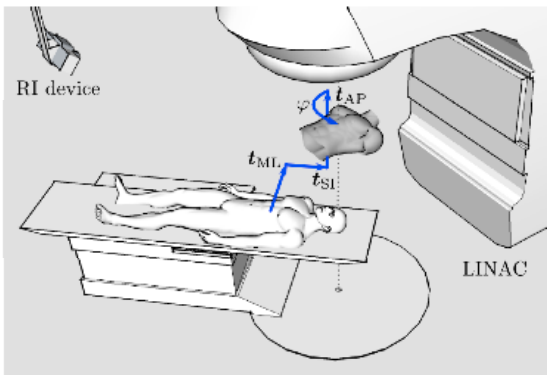
\includegraphics[scale=0.5]{images/celingkinectconfig.PNG}
    \caption{A celing mounted Kinect for the purposes of calibrating patients for CT scanning.}
\end{center}
\end{figure}

Interestingly, the authors suggest that the use of additional Kinect devices or alternative scanning configuration in this instance would provide more accurate and consistent volume measurement. An addendum to the further work possible is the use of the Kinect as a celing-mounted volume estimation pre-requisite before a patient undergoes CT scanning so that the appropriate radiation dosage is administered. Additionally, an implementation that is able to take account of positional differences/angles and calculate volume more robustly as a result is considered.

\subsection{Visual Weight Estimation}

Estimating weight using conventional computer vision techniques has traditionally relied on complex classification methods for the determination of particular parts of the body. In space, the context in which measuring the mass of a person does not have the luxury of a constant gravity for traditional methods, Verlado and Dugelay \cite{Veraldo2012} devised a system that used the offline labelling and determination of anthropometric measures to estimate overall body mass using linear regression methods. Work by Paleria and Araino \cite{Paleria2011} aimed to improve upon anthropometric identification and mass calculation with the additional identification of gender and age which influences the overall mass of a person and their siri ratio using machine learning methods such as neural networks to determine these variables. \\

The Kinect is used to take the labelling of anthropometric measures \emph{online} and hence using the NITE framework\footnote{The `standard' framework for 3D Sensing, \emph{http://www.openni.org/}} included in the API of the software, identify and track these areas of the body. The weight of the person is estimated by computing the lengths of the limbs and calculating their relevant circumferences, applying a median filter over repeated measures to reduce the influence of the offset, or shadowing, produced by the 3D sensor. The presence of noise due to sensor flickering or subject movement is considered and extrapolation factors, calculated through repeated trials, is suggested for the more accurate measurement and representation of circumferences for the arms, legs and waist.\\

Veraldo and Dugelay are able to calculate the weight determined by the Kinect sensor by utilising a statistical model trained on a large medical database of anthropometric measures that returns accurate mass representations of queried limbs within a certain tolerance, +/- 2.7cm typically for arm circumference measurement \cite{Paleria2011}. Access to a medical database of such size isn't feasible in this project and our concern with the calculation of volume and limb circumference rather than mass directly means the project could easily make use of a model with little additional development overhead. \\

\subsection{Whole Body Scanning}

One area which has seen particular development concentration is the concept of 3D Body scanning for rapid prototyping of avatars and for the purposes of editing and sharing of 3D models in specialised modelling applications such as Autodesk. Cui et al have designed a scanning pipeline and kinect configuration which is able to generate 3D models from Kinect Input data and utilise super-resolution, a class of techniques that can be used to improve the resolution of an imaging system, to improve the resolution of the Kinect images. The have also utilised a non-rigid method of registration between captured point clouds to form an accurate visual representation of the scanned subject \cite{Cui2012}. Unlike some body scanning implementations, Cui et al use a configuration which requires the subject to rotate 360\degree on the spot in a 'T' position. Registration between frames is calculated using a maximum-likelihood formulation and iterative expectation maximization to align scans based on probabilistic examination of correspondence between their points. The model is then rendered using a textured depth map. There are an increasing number of commercial and open source applications, particularly through the OpenNI \cite{openNi13} initiative which are using range imaging for full scale body rendering. \\


\newpage
\section{Summary}
This section summarises the above research.\\

\subsubsection{Person Isolation}
MOG \cite{Stauffer1999} and KDE \cite{Elgammal2000} will be the methods attempted to be implemented later. These two were chosen because their high accuracy and low computation complexity. \\

\subsubsection{Point Cloud Registration}
There are two main methods currently used for registration and ICP has demonstrated to be more flexible and reliable in the domains for which it is intended on being used \cite{chen92}. Hence, this will be the registration method used throughout the design phase of this project. \\

\subsubsection{Volume Estimation}
Step-Section Planimetry \cite{K1991} will be the basis for volume estimation and will use the Shoelace formula \cite{Pretzsch2009} to calculate the necessary metrics. If required, Gift-Wrapping \cite{Cormen2001} will be used to determine a convex hull. \\

\subsubsection{Limb Circumference}

Adapting the step-section planimetry methods cited in the Volume Estimation, Limb circumference will be calculated by taking the circumference of these planes using the Gift-wrapping method \cite{Cormen2001}. Firstly however the representative point clouds will be partitioned in a novel application of the Kinect Skeleton SDK to point cloud space. \\

\subsubsection{Markerless Recognition}

Our markerless recognition functionality has explored a number of algorithms suitable for the use of detecting a sensor in a noisy image space. As a result of these findings and our prototyping of several solutions we have opted to use blob detection using the RGB color space, in a simplification similar to the efforts of Ma and Ming. \cite{blob_detection_MingMa} \\